\documentclass[12pt,a4paper,oneside]{article}

% \usepackage[a4paper,left=1cm,right=1cm,top=2.5cm,bottom=2.5cm]{geometry}
\usepackage{fullpage}
\usepackage{amsmath}
\usepackage{blindtext}
\usepackage{titlesec}
\usepackage{hyperref}
\usepackage{graphicx}

\author{Uri Arev}
\title{Quick AREE notes}
\date{}

\graphicspath{ {./images} }

\begin{document}
\maketitle
\tableofcontents
\begin{abstract}
	\begin{center}
		(AREE = Amateur Radio Electrical Engineering)
	\end{center}

	This paper started as an idea to create a "quick amateur radio cheat sheet". It then quickly began to turn into a summary of the mathematics and physics (related to EE \& RF) that I learned whilst studying for the exams.
\end{abstract}
\section{Common Symbols}
\begin{itemize}
	\item \Large{\(j = \sqrt{-1}\)}, \(j\) in electrical engineering is the same as \(i\) in normal mathematics
\end{itemize}
\section{Ohm's Law}
Ohm's law states that the current through a conductor between two points is directly proportional to the voltage across the two points. Introducing the constant of proportionality, the resistance, one arrives at the usual mathematical equation that describes this relationship.
\[
	I = \frac VR
\]
\textbf{Example Question:} What is the current in a 20V circuit if the resistance is \(10\Omega\)?
\section{Alternating Current}
Alternating currents are accompanied (or caused) by alternating voltages. An AC voltage \(v\) can be described mathematically as a function of time by the following equation:
\[
	v(t) = V_{peak} sin(\omega t),
\]
where
\begin{itemize}
	\item \(V_{peak}\) is the peak voltage
	\item \(\omega\) is the angular frequency (\(\omega = 2 \pi f\))
	\item \(t\) is the time (seconds)
\end{itemize}

The peak-to-peak voltage is usually written as \(V_pp\) or \(V_{P\text-P}\)
\section{Resistors, Inductors And Capacitors In Series And In Parallel}
\subsection{In Series}
\subsubsection{Resistors}
% \begin{center}
% 	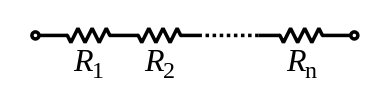
\includegraphics[scale=0.4]{resistors_in_series.png}
% \end{center}
Resistors in series act as a single resistor. When breaking the connections between the resistors at any point in the circuit, the circuit will "open", and will stop operating.
\[
	R_{total} = R_1 + R_2 + \cdots + R_n
\]
\subsubsection{Inductors}
Inductors follow the same law, in that the total inductance of non-coupled inductors in series is equal to the sum of their individual inductances:
\[
	L_{total} = L_1 + L_2 + \cdots + L_n
\]
\subsubsection{Capacitors}
The total capacitance of capacitors in series is equal to the reciprocal of the sum of the reciprocals of their individual capacitances:
\[
	\frac{1}{C_{total}} = \frac{1}{C_1} + \frac{1}{C_2} + \cdots + \frac{1}{C_n}
\]
\subsection{In Parallel}
\subsubsection{Resistors}
To find the total resistance of all components, add the reciprocals of the resistances \(R_i\) of each component and take the reciprocal of the sum. Total resistance will always be less than the value of the smallest resistance:
\[
	\frac{1}{R_{total}} = \frac{1}{R_1} + \frac{1}{R_2} + \cdots + \frac{1}{R_n}
\]
\subsubsection{Inductors}
Inductors follow the same law, in that the total inductance of non-coupled inductors in parallel is equal to the reciprocal of the sum of the reciprocals of their individual inductances:
\[
	\frac{1}{L_{total}} = \frac{1}{L_1} + \frac{1}{L_2} + \cdots + \frac{1}{L_n}
\]
\subsubsection{Capacitors}
The total capacitance of capacitors in parallel is equal to the sum of their individual capacitances:
\[
	C_{total} = C_1 + C_2 + \cdots + C_n
\]
\section{Reactance}
In electrical circuits, reactance is the opposition presented to alternating current by inductance and capacitance. Greater reactance gives smaller current for the same applied voltage. Reactance is similar to resistance in this respect, but does not lead to dissipation of electrical energy as heat; instead, energy is momentarily stored in the reactance, and a quarter-cycle later returned to the circuit.
\subsection{Capacitive Reactance}
There are two choices in the literature for defining reactance for a capacitor. One is to use a uniform notion of reactance as the imaginary part of impedance, in which case the reactance of a capacitor is the negative number:
\[
	Xc = -\frac{1}{\omega C} = -\frac{1}{2 \pi f c}
\]
We may also choose to define capacitive reactance as a positive number:
\[
	Xc = \frac{1}{\omega C} = \frac{1}{2 \pi f c}
\]
In this case however we need to remember to add a negative sign for the impedance of a capacitor, i.e. \(Z_c = -jX_c\).
\subsection{Inductive Reactance}
Inductive reactance \(X_{L}\) is proportional to the signal frequency \(f\) and the inductance \(L\) (which depends on the physical shape and dimensions of the inductor):
\[
	X_L = \omega L = 2 \pi f L
\]

With all of the information we know about reactance, we can calculate a simple circuit's \textit{Impedance}.
\section{Impedance}
Impedance is the opposition to alternating current (AC) presented by a circuit containing and combining the effects of reactance and resistance. \\
\textbf{For Example:} let's create a simple circuit containing the following values, assuming all components are in series:
\begin{align*}
	R_{total} &= 20\Omega \\
	C_{total} &= 25\text{mF} \\
	L_{total} &= 10\text{mH} \\
	f &= 60\text{Hz}
\end{align*}

Now, let's calculate the reactance.
\begin{align*}
	X_C = \frac{1}{\omega C} = \frac{1}{2 \pi f C} = \frac{1}{2 \pi \times 60 \times 0.025} &= 0.106\Omega \\
	X_L = \omega C = 2 \pi f L = 2 \pi \times 60 \times 0.01 &= 3.769\Omega
\end{align*}
When both a capacitor and an inductor are placed in series in a circuit, their contributions to the total circuit impedance are opposite. Capacitive reactance \(X_C\) and inductive reactance \(X_L\) contribute to the total reactance \(X\) as follows:
\[
	X = X_L + X_C = \omega L + \frac{1}{\omega C}
\]
Hence:
\begin{itemize}
	\item if \(X>0\), the total reactance is said to be inductive,
	\item if \(X=0\), the total reactance is purely resistive,
	\item if \(X<0\), the total reactance is said to be capacitive.
\end{itemize}
Note however that if \(X_L\) and \(X_C\) are assumed both positive by definition, then the intermediary formula changes to a difference:
\[
	X = X_L - X_C = \omega L - \frac{1}{\omega C}
\]
Both values are positive, so we would use the formula above:
\[
	X = X_L - X_C = \omega L - \frac{1}{\omega C} = 3.769\Omega - 0.106\Omega = 3.663\Omega
\]
to calculate impedance of a series circuit, we use the following formula:
\[
	Z = \sqrt{R^2 + X^2}
\]
where \(R^2\) is the total resistance squared, and \(X^2\) is the total reactance squared.

Using the formula above to calculate the total impedance \(Z\) in our circuit, we get the following result:
\[
	Z = \sqrt{R^2 + X^2} = \sqrt{20\Omega^2 + 3.663\Omega^2} = 20.332\Omega
\]
\end{document}
